\documentclass[conference]{IEEEtran}
%\IEEEoverridecommandlockouts
% The preceding line is only needed to identify funding in the first footnote. If that is unneeded, please comment it out.
\usepackage{cite}
\usepackage{amsmath,amssymb,amsfonts}
\usepackage{algorithmic}
\usepackage{graphicx}
\usepackage{textcomp}
\usepackage{xcolor}
\def\BibTeX{{\rm B\kern-.05em{\sc i\kern-.025em b}\kern-.08em
    T\kern-.1667em\lower.7ex\hbox{E}\kern-.125em}}
\usepackage{float}
\usepackage{hyperref}
\hypersetup{
    colorlinks=true,
    % linkcolor=blue,
    % filecolor=magenta,      
    % urlcolor=cyan,
    pdftitle={16824 Project Proposal},
    %pdfpagemode=FullScreen,
}
% \urlstyle{mono}


\begin{document}

\title{Self-Supervised Action Recognition In The Dark\\
{\small CMU 16824 Project Proposal, Group ID: 14, \today }
%{\footnotesize \textsuperscript{*}Note: Sub-titles are not captured in Xplore and should not be used}
%\thanks{Identify applicable funding agency here. If none, delete this.}
}

\author{
    \IEEEauthorblockN{Meghana Reddy Ganesina}
    \IEEEauthorblockA{\textit{MSCV, RI} \\
    \textit{Carnegie Mellon University}\\
    %City, Country \\
    mganesin@andrew.cmu.edu}
    \and
    \IEEEauthorblockN{Nitheesh Lakshminarayanappa}
    \IEEEauthorblockA{\textit{MSCV, RI} \\
    \textit{Carnegie Mellon University}\\
    nlakshmi@andrew.cmu.edu}
    \and
    \IEEEauthorblockN{Sri Nitchith Akula}
    \IEEEauthorblockA{\textit{MSCV, RI} \\
    \textit{Carnegie Mellon University}\\
    srinitca@andrew.cmu.edu}
}

\maketitle

\begin{abstract}
Action Recognition (AR) has gained large improvements with the introduction of large-scale video datasets and the development of deep neural networks. However, AR models robust to challenging environments in real-world scenarios are still under-explored. We focus on the task of video-based action recognition in dark environments, which can be applied to fields such as surveillance and autonomous driving at night. Through this project, we intend to particiapte in the $UG^{2}+$ Challenge Track 2 (UG2-2)\cite{UG2-2} which evaluates the robustness of action recognition methods in dark environments. Code will be published at \url{https://github.com/nitheeshkl/s2arid}
\end{abstract}

\vspace{10pt}

\begin{IEEEkeywords}
self-supervision, action recognition, ARID, low-light Images/Videos
\end{IEEEkeywords}

\section{Introduction}
The rapid development of computer vision algorithms increasingly allows automatic visual recognition to be incorporated into a suite of emerging applications. Some of these applications have less-than-ideal circumstances such as low-visibility environments, causing image captures to have degradations. With the advances in computer vision technologies, especially video-based technologies, various automatic video-based tasks have received considerable attention. There have been increasing applications of these technologies in various fields, which include surveillance and smart homes. The advances can be credited in part to a rising number of video-based datasets, designed for a range of video-based tasks such as action recognition (AR), localization and segmentation. Although much progress has been made, the progress is mostly limited to videos shot under “clear” environments, with normal illumination and contrast. Such limitation is partly due to the fact that current benchmark video-based datasets are collected from either crowd-sourcing platforms or from public web video platforms directly. Either source contains mostly “clear” videos, where the actions are identifiable. However, there has been an increasing number of scenarios where videos shot under normal illumination may not be available. One notable scenario is night security surveillance, where security cameras are usually placed at alleys or fields with little lighting. The actions captured are hard to identify even by the naked eye. Although additional sensors, such as infrared imaging sensors, could be utilized for recognizing action in these environments, their cost prohibits the large scale deployment of these sensors. It is therefore greatly beneficial to explore possible video-based technologies that are robust to darkness, extracting effective action features from dark videos, which would benefit in various downstream applications.

Over the past few years, there has been a remarkable rise of research interest with regards to computer vision tasks in dark environments, which include dark face recognition and dark image enhancement. More recently, such research interests have been expanded to the video domain, especially towards darkness enhancement. However, it is noted that under image domain, visually enhanced dark images may not result in better classification accuracies when the same techniques are applied. Therefore it seems uncertain if the visually enhanced videos could necessarily result in better action recognition accuracies. Furthermore, with massive publicly available clear videos, it also seems promising to utilize them in some way, with possible pre-processing or post-processing steps, to capture actions with high robustness towards darkness.

In this project, we aim to tackle robust video-based action recognition with special focus on dark videos utilizing self-supervised algorithms which could utilize both clear videos and dark videos. We intend to participate in the $UG^{2}+$ Challenge Track 2 (UG2-2)\cite{UG2-2} which evaluates the robustness of action recognition methods in dark environments.

\section{Related Work}
In the era of deep learning, early state-of-the-art methods for AR were fully supervised methods. However, fully supervised methods relies mainly on large-scale labeled datasets and suffer from poor transferability and generalization. To address these issues, recent works proposed semi-supervised approached such as self-supervised learning and Unsupervised Domain Adaptation (UDA). The following sections highlights some of the related works in these categories for AR.

\subsection{Fully Supervised Methods}
Early state-of-the-art methods using full supervision for AR were based on 2D CNNs\cite{Karpathy2014LargeScaleVC} or 3D CNNs\cite{Ji20133DCN}. 2D-based methods lacked temporal features and hence early methods \cite{Simonyan2014TwoStreamCN} required additional hand-crafted features as input (ex: optical flow) to represent the temporal information. More recent methods like Temporal Spatial Networks \cite{Wang2016TemporalSN} and Slow-Fast Networks \cite{Feichtenhofer2019SlowFastNF} attempt to model the temporal information in a learnable manner. Whereas 3D CNNs attempts to jointly extract the spatio-temporal features by expanding the the 2D convolutional kernel to the temporal dimension, while this expansion suffers from high computational cost. Subsequent works like P3D \cite{Qiu2017LearningSR} and R(2+1) \cite{Tran2018ACL} improve the efficiency by replacing 3D convolutional kernels with pseudo 3D kernels.

\subsection{Self-Supervised Methods}
Self-supervised learning methods are designed to extract effective video representation from unlabeled data. The basis of self-supervision is to design a pretext task to generate supervision signals through the characteristic of videos, such as frame orders and play rates. Pace-Prediction method by Wang et al.\cite{Wang2020SelfsupervisedVR} introduce contrastive learning to push the model towards discriminating different paces by maximizing the agreement on similar video content. Fernando et al. introduced "odd-one-out learning" \cite{Fernando2017SelfSupervisedVR} where subsequences from videos are presented and the network is asked to learn to predict the odd video sequence. Jing et al. \cite{Jing2018SelfSupervisedSF} proposed  pretext task to predict the rotation of randomly rotated videos.

\subsection{Unsupervised Domain Adaptation (UDA)}
UDA aims to extract the transferable representations across the labeled data in the source domain and the unlabeled data in the target domain. While there has been a lot of work in image-based UDA, there exists fewer targeted at video-based UDA. Temporal Co-attention Network (TCoN) by Pan et al. \cite{Pan2020AdversarialCA} introduce novel a novel cross-domain co-attention mechanism to match the distributions of temporally aligned action features between source and target domains. Multi-Modal Domain Adaptation by Munro et al. \cite{Munro2019MultiModalDA} exploits the correspondence of modalities as a self-supervised alignment approach for UDA in addition to adversarial alignment. Xu et al. introduce Partial Adversarial Temporal Attentive Network (PATAN) \cite{Xu2021PartialVD} to address the partial video domain adaptation problem by utilizing both spatial and temporal features for filtering source-only classes.

\section{Our Approach}
For pretext task-based methods, one or several tasks are used to train the network in a supervised manner. For example, rotation, pace-prediction, or similar transformations that take advantage of the spatio-temporal feature of the video input. The representations learnt from these pretext tasks are then used for downstream tasks like object recognition, tracking etc. We define our downstream tasks the action recognition in the given dark videos. For this, we propose the following techniques

\subsection{Contrastive Learning}
In this approach, we generate day-light and low-light video pairs through i) existing low-light enhancement networks on low-light videos and/or ii) domain transfer of day-light videos to low-light using CycleGAN based networks. We consider the combination of day-light and low-light videos of same action as positive samples and the combination of day-light and low-light pairs from different actions as negative samples. This should enable the network to learn feature embedding in the latent space such that the inputs are clustered according to their classifications. Then we can combine low-light and day-light data to perform action recognition task and we hypothesize that it should improve performance for the low-light data.

\subsection{Pretext Tasks}
Random Video Inpainting\textendash Given a video clip $I_N$ with $N$ frames, a random frame $f_n$ is selected to be in-painted by the network. The region to be painted in the frame $f_n$ is created by a random crop. The network should learn to paint the frame $f_n$ such that the frame matches with the set of previous frames $(f_0, f_{n-1})$ and the set of future frames $(f_{n+1}, f_N)$. 

Random Rotation in Video Frames\textendash Given a video clip $I_N$ with $N$ frames and each frame $f_i$ rotated by a random rotation $\theta$, the network is tasked to predict the correct original rotation of each rotated frame such that the entire video clip is played in the correct original order.

\vspace{8pt}

\textbf{Hypothesis}\textendash Our assumption is that a network is not capable to perform such pretext tasks effectively unless it understands the video content and learns powerful spatio-temporal representations. To avoid pretext tasks from taking shortcuts (as pointed by \cite{Doersch2015UnsupervisedVR}), we intend to use color jittering augmentation to avoid such shortcuts.

\section{Datasets}
ARID \cite{Xu2020ARIDAN} is our primary dataset. The dataset is a collection of videos shot by commercial cameras in dark environments, with
actions performed by 11 volunteers. In total, it comprises 11 action classes (Fig\ref{figARIDSample}), including both \textit{Singular Person Actions} (i.e., jumping, running, turning, walking, and waving) as well as \textit{Actions with Objects} (i.e., drinking, picking, pouring, pushing, sitting, and standing). The dark videos are shot in both indoor and outdoor scenes with varied lighting conditions. The dataset consists of a total of 3,784 video clips, with the minimum action class containing 205 video clips. The clips of every action class are divided into clip groups
according to the different actors and scenes. Three train/test splits are provided, with each split partitioned according to the clip groups, with a ratio of $7 : 3$. All video clips in ARID are fixed to a 30 FPS frame rate, and a unified resolution of 320 × 240. The overall duration of all video clips combined is 8,721 seconds.

Since self-supervised approaches benefit from large collections of unlabeled data, we intend to use other video datasets like HMDB51\cite{Kuehne2011HMDBAL}, UFC101\cite{Soomro2012UCF101AD}, Kinetics-600\cite{Kay2017TheKH}, and Moments-in-Time\cite{Monfort2020MomentsIT}, that includes a total of 2,625 videos from 11 classes (drink, jump, pick, pour, push, run, sit, stand, turn, walk, and wave) to augment ARID and better generalize our models.

\begin{figure}[ht]
\centerline{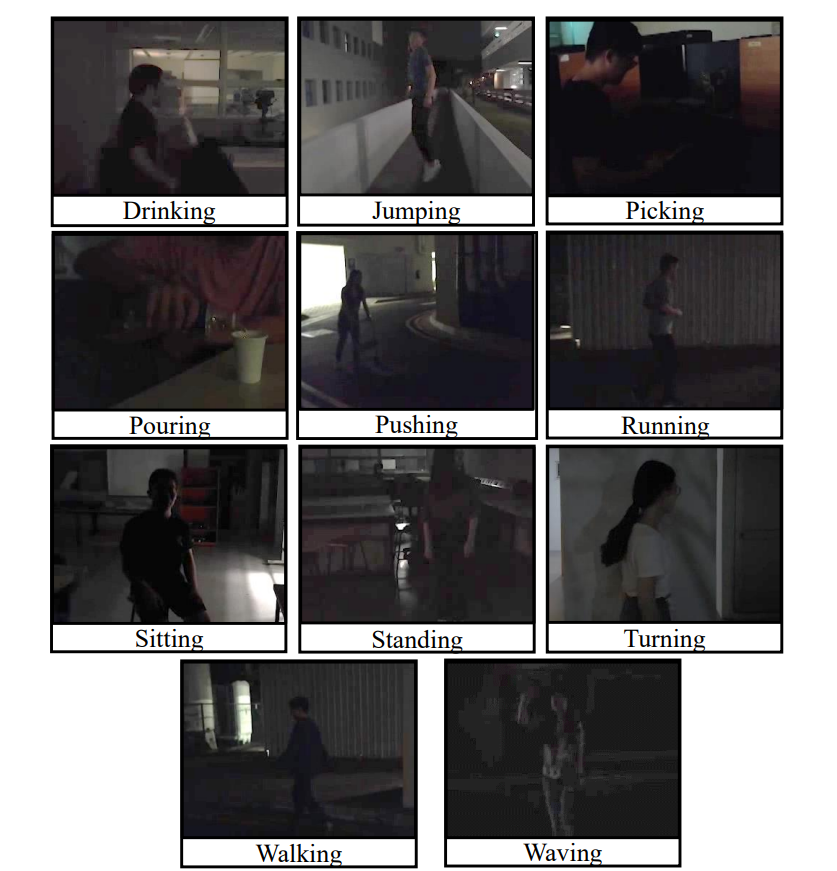
\includegraphics[width=0.5\textwidth]{arid_dataset_sample.png}}
\caption{Sample frames for each of the 11 action classes of the ARID dataset.}
\label{figARIDSample}
\end{figure}


\section{Experiments}

\subsection{Evaluation}
The UG2-2 challenge provides an evaluation server to evaluate our models. The evaluation and ranking criteria is i) \textit{Top-1 Accuracy} on the testing set and ii) \textit{Cross-Entropy Loss} with respect to the ground truth label of the testing set. We use the same evaluation metrics for our experiments.

\subsection{Baselines}
The ARID dataset provides several baselines, of which we intend to use two baselines. We use I3D-TS\cite{Carreira2017QuoVA} to represent Two-stream method and 3D-ResNext-101\cite{Hara2018CanS3} to represent 3D-CNNs. Table\ref{tabARIDBaeline} highlights their performance on the ARID dataset.

\begin{table}[H]
\caption{Performance of two-stream and 3D-CNN based models on ARID dataset.}
\begin{center}
\begin{tabular}{|c|c|c|c|}
\hline
& \textbf{Models} & \textbf{Top-1 Accuracy} & \textbf{Top-5 Accuracy}\\
\hline 
\textbf{Two-stream} & ID3-TS & $72.78\%$ & $99.39\%$ \\
\hline
\textbf{3D-CNN} & 3D-ResNext-101 & $74.73\%$ & $98.54\%$ \\
\hline
\multicolumn{4}{l}{$^{\mathrm{*}}$performance measures obtained from original ARID dataset paper.}
\end{tabular}
\label{tabARIDBaeline}
\end{center}
\end{table}

%\clearpage

\bibliographystyle{IEEEtran}
\bibliography{refs.bib}

\end{document}
